\chapter{BIPEDAL WALKING BY TWIN DELAYED DEEP DETERMINISTIC POLICY GRADIENTS}
\label{chap:exp_setup}

\section{Details of the Environment}
\textit{Bipedal-Walker-v3} and \textit{Bipedal-Walker-Hardocore-v3} are simulation environments of a bipedal robot, with relatively flat course and obstacle course respectively. Dynamics of the robot are exactly identical in both environments. Our task is to solve hardcore version where the agent is expected to learn to run and walk in different road conditions. Components of the hardcore environment is visualized in \figref{fig:bipedal_hardcore_components}. \\
\begin{figure}
	\centering
	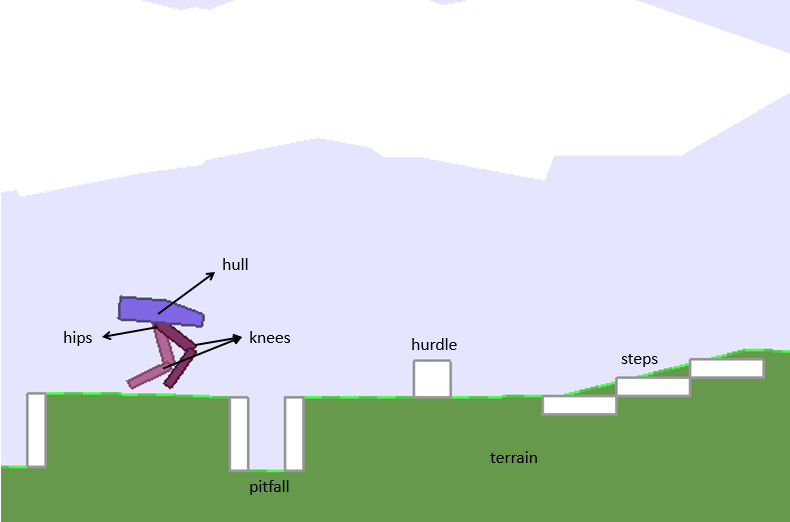
\includegraphics[width=0.95\textwidth]{figures/bipedal/bpedal_annotated.png}
	\caption{Bipedal Walker Hardcore Components}
	\label{fig:bipedal_hardcore_components}
\end{figure}
The robot has kinematic and lidar sensors. It is modeled as Markov Decision Process with deterministic dynamics. \\
\textbf{Observation Space}: Hull angle, hull angular velocity, translational velocity on two dimension, joint positions, joint angular speeds, leg ground concats and 10 lidar rangefinder measurements. Details are summarized at Table \ref{table:bpw_obs_space}. \\
\begin{table}[h!]
	\begin{center}
	\begin{tabular}{cccc}
		\textbf{Num} & \textbf{Observation} & \textbf{Interval} \\
		\hline 
		0  & Hull Angle & $[-\pi,\pi]$ \\
		1  & Hull Angular Speed & $[-\infty,\infty]$ \\
		2  & Velocity x & $[-1,1]$ \\
		3  & Velocity y &$[-1,1]$ \\
		4  & Hip 1 Joint Angle & $[-\infty,\infty]$ \\
		5  & Hip 1 Joint Speed & $[-\infty,\infty]$ \\
		6  & Knee 1 Joint Angle & $[-\infty,\infty]$ \\
		7  & Knee 1 Joint Speed & $[-\infty,\infty]$ \\
		8  & Leg 1 Ground Contact Flag & $\{0,1\}$ \\
		9  & Hip 2 Joint Angle & $[-\infty,\infty]$ \\
		10  & Hip 2 Joint Speed & $[-\infty,\infty]$ \\
		11  & Knee 2 Joint Angle & $[-\infty,\infty]$ \\
		12  & Knee 2 Joint Speed & $[-\infty,\infty]$ \\
		13  & Leg 2 Ground Contact Flag & $\{0,1\}$ \\
		14-23  & Lidar measures  & $[-\infty,\infty]$
	\end{tabular}
	\end{center}
	\caption{Observation Space of Bipedal Walker}
	\label{table:bpw_obs_space}
\end{table}
\textbf{Action Space}: The robot has 2 legs with 2 joints at knee and hip. Torque provided to knee and pelvis joints of both legs. Details are presented in Table \ref{table:bpw_act_space}. \\
\begin{table}[h!]
	\begin{center}
		\begin{tabular}{cccc}
			\textbf{Num} & \textbf{Observation} & \textbf{Interval} \\
			\hline
			0  & Hip 1 Torque & $[-1,1]$ \\
			1  & Hip 2 Torque & $[-1,1]$ \\
			2  & Knee 1 Torque & $[-1,1]$ \\
			3  & Knee 2 Torque & $[-1,1]$ \\
		\end{tabular}
	\end{center}
	\caption{Action Space of Bipedal Walker}
	\label{table:bpw_act_space}
\end{table}
\textbf{Rewarding}: The robot should run fast with little energy while should not stumble and fall to ground. Therefore reward is shaped accordingly. Directly proportional to distance traveled forward, +300 points given if agent reaches end of path. -10 points (-100 points in original version)  if agent falls, and small amount of negative reward proportional to applied motor torque (preventing applying unnecessary torque). Lastly, the robots gets negative reward propotional to absolut value of hull angle for reinforcing to keep hull straigth. \\
\subsection{Partial Observability}
The environment is partially observable due to following reasons.
\begin{itemize}
	\item The agent is not able to track behind with lidar sensor. Unless it has a memory, it cannot know whether a pitfall or hurdle behind. Illustration is shown in x.
	\item There is no accelerometer sensor. Therefore, the agent do not know whether it is accelerating or decelerating.
\end{itemize}
\begin{figure}
	\begin{subfigure}{.32\textwidth}
		\centering
		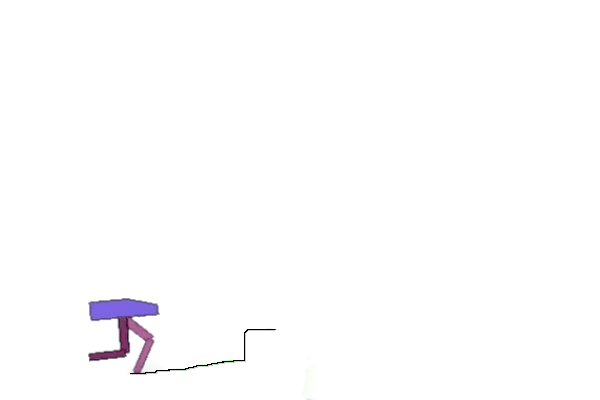
\includegraphics[width=0.99\linewidth]{figures/bipedal/po/lidarcover.png}
		\caption{Perspective}
		\label{fig:lidar_cover}
	\end{subfigure}
	\begin{subfigure}{.32\textwidth}
		\centering
		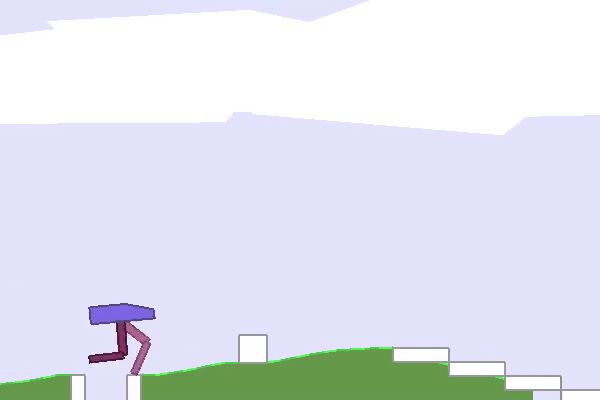
\includegraphics[width=0.99\linewidth]{figures/bipedal/po/pitfall_behind.png}
		\caption{Pitfall Behind}
		\label{fig:pitfall_behind}
	\end{subfigure}
		\begin{subfigure}{.32\textwidth}
		\centering
		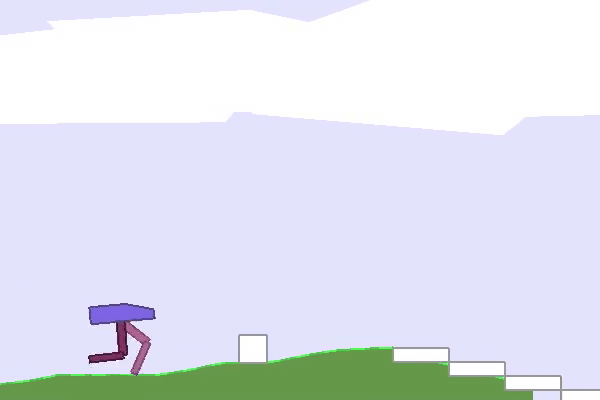
\includegraphics[width=0.99\linewidth]{figures/bipedal/po/no_pitfall_behind.png}
		\caption{No Pitfall Behind}
		\label{fig:no_pitfall_behind}
	\end{subfigure}
	\caption{Perspective of agent and possible realities}
	\label{fig:partial_obs_pitfall}
\end{figure}
In DRL, partial observability is handled by 2 ways in literature \cite{dulac-arnold_challenges_2019}. First is incorprating fixed number of last observations while second way is updating hidden belief state using recurrent neural network at each time step. Our approach is using fixed number of past observation into LSTM and Transformer based networks for both actor and critic networks. \\
\subsection{Reward Sparsity}
Rewards given to the agent is sparse in some circumstances. 
\begin{itemize}
	\item Overcoming big hurdles requires a very specific move. The agent should explore many actions when faced with a big hurdle.
	\item Crossing pitfalls also require a specific move but not as complex as big hurdles.
\end{itemize}
\subsection{Modifications on Original Envrionment}
It is difficult to solve directly available environment as it is. Therefore, there are few works on the literature demonstrating a solution. 
\begin{itemize}
	\item In original version, agent gets -100 points when its hull hits the floor. In order to make the robot more greedy, this is changed to -10 points. Otherwise, agent cannot explore environment since it gets too much punisment when failed.
	\item Time frequency of simulation is halved (from 50 Hz to 25 Hz) by only observing last of each two consecutive frames using a custom wrapper function. Since there is not a high frequency dynamics, this allows nothing but speeding up the learning process.
	\item In original implementation, an episode has time limit. Once this limit is reached, simulation stops with terminal flag. On the other hand, when agent fails before time limit, the episode ends with terminal flag too. In first case, the terminal flag causes instability since next step's value is not used in value update. The environment changed such that terminal flag is not given in this case unless agent fails.
\end{itemize}
\section{Proposed Neural Networks}
For all networks, varing backbones used to encode state information from observations for both actor and critic networks. In critic network, actions are concatenated by state information coming from backbones. Then, this concatenated vector is passed through feed forward layer with GELU activation then a linear layer with single output. Before feeding observations to backbone, they are passed through a layer with layer normalization with tanh activation to 96 dimensional output. In actor network, backbone is followed by a single layer with tanh activation for action estimation. As backbones, following networks are proposed. Again, observations are passed through a layer with layer normalization with tanh activation to 96 dimensional output before feeding to backbone. Critic and Actor networks are illustrated in \figref{fig:nets} \\
\begin{figure}
	\begin{subfigure}{.5\textwidth}
		\centering
		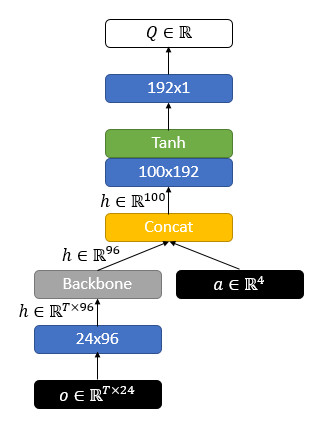
\includegraphics[width=0.97\linewidth]{figures/nets/critic.png}
		\caption{Critic Architecture}
		\label{fig:critic_net}
	\end{subfigure}
	\begin{subfigure}{.5\textwidth}
		\centering
		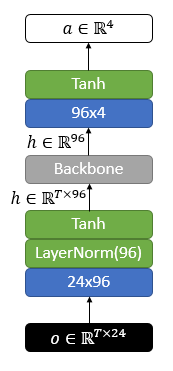
\includegraphics[width=0.55\linewidth]{figures/nets/actor.png}
		\caption{Actor Architecture}
		\label{fig:actor_net}
	\end{subfigure}
	\caption{Neural Architecture Design}
	\label{fig:nets}
\end{figure}
\subsection{Residual Feed Forward Network}
Incoming vector is passed through 2 layers with 192 dimensional hidden size and 96 dimensional output, where there is GELU activation between 2 layers. This output is summed with initial vector and this is lastly passed through layer normalization. \\
\subsection{Long Short Term Memory}
Sequence of incoming vectors is passed though vanilla lstm layer with 96 dimensional hidden state. Output at last time step is outputted. \\
\subsection{Transformer (Pre-layer Normalized)}
Sequence of incoming vectors is passed though pre-layer normalized transformer with 192 dimensional feed forward layer with GELU activation. The output is lastly passed through layer normalization. During multi-head attention, only last state is fed as query so that attentions are calculated for only last state. \\
\section{RL Method and hyperparameters}
TD3 is used as RL algorithm. Hyperparameters are selected by grid search and best performing values are used. Adam optimizer is used as optimizer. \\
As exploration noise, Ornstein-Uhlenbeck noise is used and standart deviation is multiplied  by $0.999$ at the end of each episode. Initially $\theta=4.0$ and $\sigma=1.0$ are used. \\
Other hyperparameters are as follows. \\
\begin{itemize}
	\item $\alpha=7.0 \cdot 10^{-4}$ (For LSTM)
	\item $\alpha=1.0 \cdot 10^{-3}$ (For Other networks)
	\item $\beta_1=0.9$
	\item $\beta_2=0.999$
	\item $\gamma=0.98$
	\item $N_{replay} = 500000$
	\item $N = 128$
\end{itemize}
%
\section{Results}
For each episode, episode scores are calculated by summing up rewards of each time step. In \figref{fig:scatter_ep_rewards}, a scatter plot is visualized for each model's episode scores. In \figref{fig:std_ep_rewards}, moving average and standard deviation is visualized for each model's episode scores. \\
\begin{figure}
	\centering
	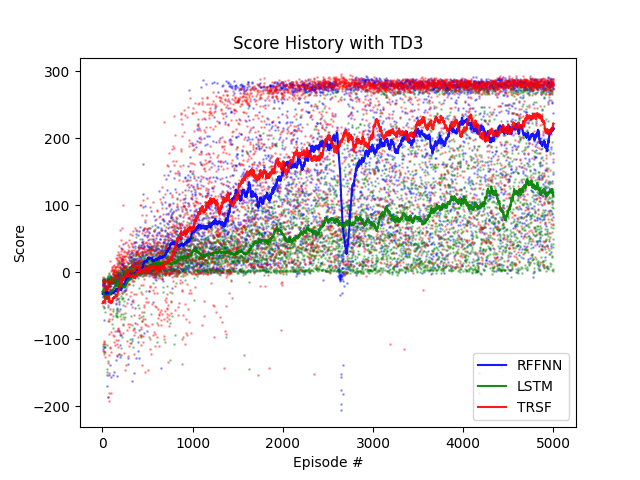
\includegraphics[width=0.95\textwidth]{figures/bipedal/SCATTER_TD3_RFFNN_LSTM_TRSF.png}
	\caption{Scatter Plot with Moving Average for Episode Scores}
	\label{fig:scatter_ep_rewards}
\end{figure}
\begin{figure}
	\centering
	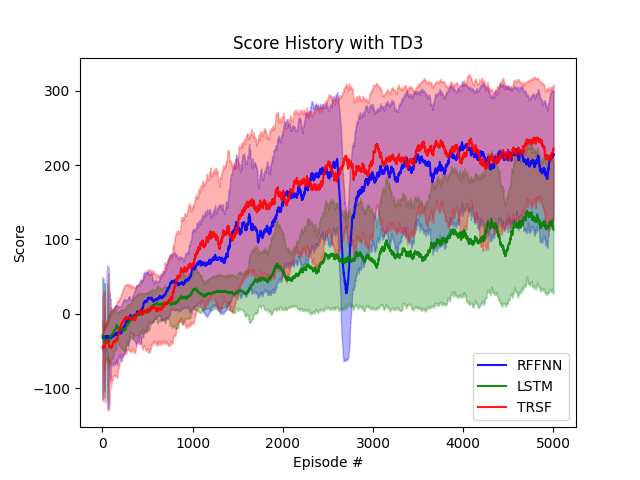
\includegraphics[width=0.95\textwidth]{figures/bipedal/STD_TD3_RFFNN_LSTM_TRSF.png}
	\caption{Moving Average and Standard Deviation for Episode Scores}
	\label{fig:std_ep_rewards}
\end{figure}
First of all, none of our approaches solved the problem since 300 points required in 100 random simulations as solution. However, our methods partially solved problems by exceeding 200 point limit, while some simulations yield around 280 points in all models. \\
RFFNN seems to be enough for solving the problem, although there exist partial observability in the environment. That model reaches around 220 points in average. \\
The robot was able to walk by LSTM model but yield worse results and cannot exceed 120 points in average. \\
Transformer model yield best results by reaching 230 points.  \\
As Transformer and RFFNN are relatively succesfull, their behavior is visualized in \figref{fig:rffnn_simulation} and \figref{fig:trsf_simulation}. The main behavior difference is when the agent faces with a big hurdle. First model passes it by jumping while other does by taking a very big step.
%
\begin{figure}
	\centering
	\begin{subfigure}{.9\textwidth}
		\centering
		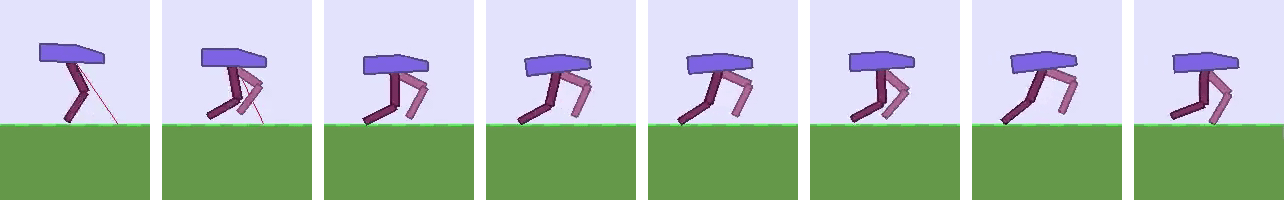
\includegraphics[width=0.99\textwidth]{figures/bipedal/anim/ff_flat.png}
		\caption{Flat Surface}
		\label{fig:anim_rffnn_flat}
	\end{subfigure}
	\begin{subfigure}{.9\textwidth}
		\centering
		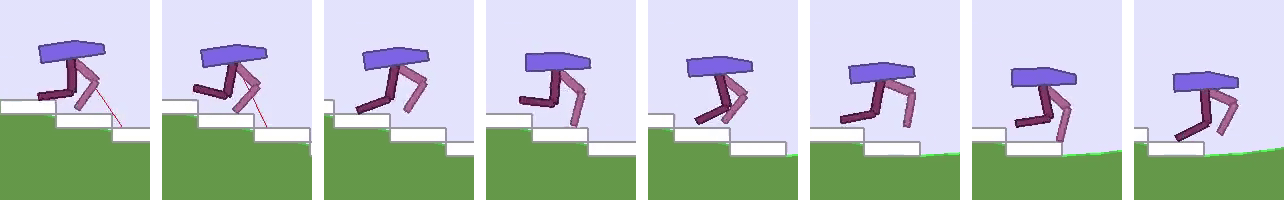
\includegraphics[width=0.99\textwidth]{figures/bipedal/anim/ff_stairs.png}
		\caption{Stairs}
		\label{fig:anim_rffnn_stairs}
	\end{subfigure}
	\begin{subfigure}{.9\textwidth}
		\centering
		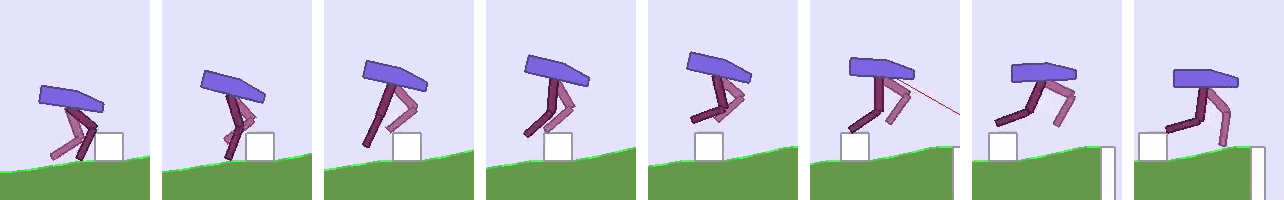
\includegraphics[width=0.99\textwidth]{figures/bipedal/anim/ff_hurdle.png}
		\caption{Hurdle}
		\label{fig:anim_rffnn_hurdle}
	\end{subfigure}
	\begin{subfigure}{.9\textwidth}
		\centering
		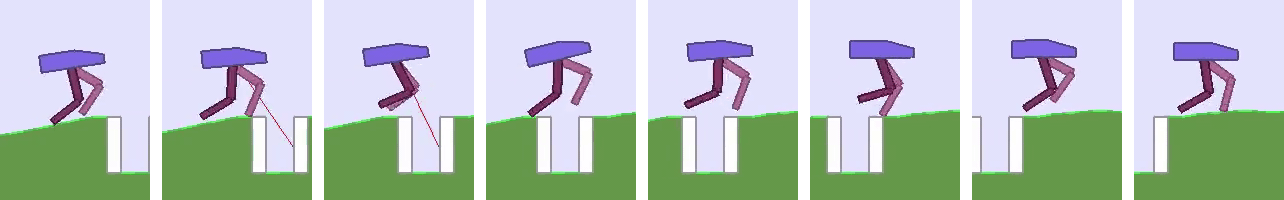
\includegraphics[width=0.99\textwidth]{figures/bipedal/anim/ff_pitfall.png}
		\caption{Pitfall}
		\label{fig:anim_rffnn_pitfall}
	\end{subfigure}
	\caption{Walking Simulation of RFFNN model at best version}
	\label{fig:rffnn_simulation}
\end{figure}
%
\begin{figure}
	\centering
	\begin{subfigure}{.9\textwidth}
		\centering
		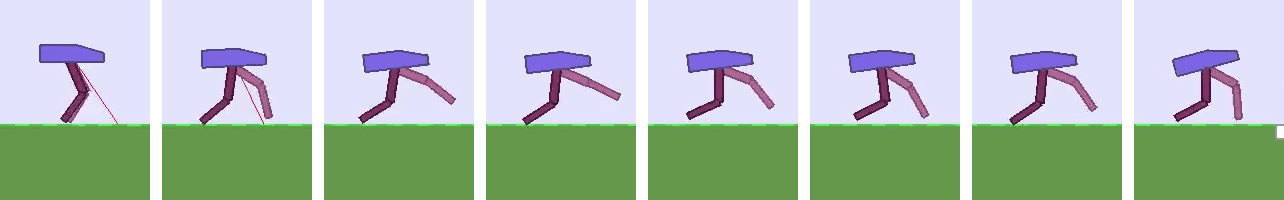
\includegraphics[width=0.99\textwidth]{figures/bipedal/anim/trsf_flat.png}
		\caption{Flat Surface}
		\label{fig:anim_trsf_flat}
	\end{subfigure}
	\begin{subfigure}{.9\textwidth}
		\centering
		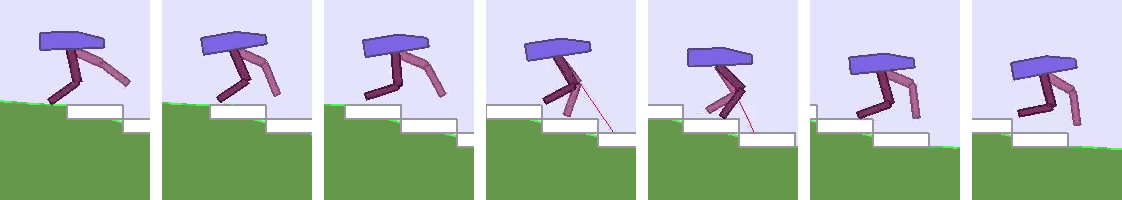
\includegraphics[width=0.99\textwidth]{figures/bipedal/anim/trsf_stairs.png}
		\caption{Stairs}
		\label{fig:anim_trsf_stairs}
	\end{subfigure}
	\begin{subfigure}{.9\textwidth}
		\centering
		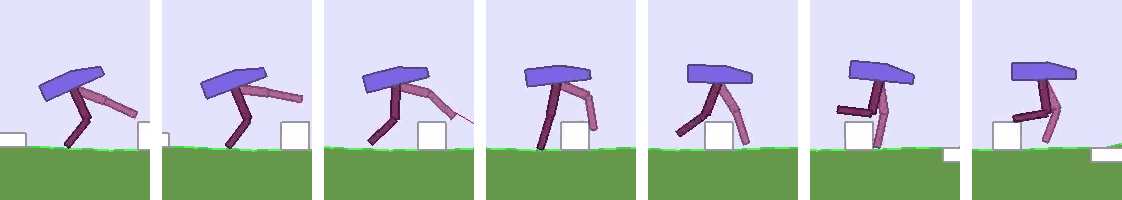
\includegraphics[width=0.99\textwidth]{figures/bipedal/anim/trsf_hurdle.png}
		\caption{Hurdle}
		\label{fig:anim_trsf_hurdle}
	\end{subfigure}
	\begin{subfigure}{.9\textwidth}
		\centering
		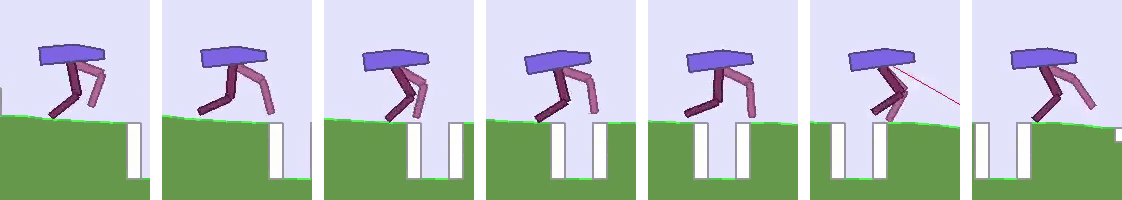
\includegraphics[width=0.99\textwidth]{figures/bipedal/anim/trsf_pitfall.png}
		\caption{Pitfall}
		\label{fig:anim_trsf_pitfall}
	\end{subfigure}
	\caption{Walking Simulation of Transformer model at best version}
	\label{fig:trsf_simulation}
\end{figure}
%
\section{Discussion}
We believe that these results are not enough to say any model is superior to another, because there are other factors such as DRL method, number of episodes, network size etc. However, networks are designed to have similar sizes and good model requires to converge in less episodes. As a result, it is possible to say that transformers are able to surpass performance of LSTMs for partially observed RL problems. Note that this is valid where layer normalization is applied before multihead attention and feed-forward layers \cite{xiong_layer_2020} as opposed to vanilla transformer proposed in \cite{vaswani_attention_2017}. \\
Another result is that incorprating past observations did not improve performance drastically, although the opposite was expected. We can interpret that either the history length is less or the partial observability is not a big deal for the agent. 